\documentclass[10pt,twocolumn]{article}

\usepackage[letterpaper,margin=0.62in]{geometry}
\usepackage{amsmath,amssymb}
\usepackage{booktabs}
\usepackage{graphicx}
\usepackage{subcaption}
\usepackage{multirow}
\usepackage[numbers,sort&compress]{natbib}
\usepackage[hidelinks]{hyperref}
\usepackage{microtype}
\usepackage{enumitem}
\usepackage{titlesec}

\setlength{\columnsep}{0.22in}
\setlength{\parindent}{0pt}
\setlength{\parskip}{2pt}
\setlist[itemize]{leftmargin=1.1em,itemsep=1pt,topsep=2pt}
\titlespacing*{\section}{0pt}{7pt}{3pt}
\titlespacing*{\subsection}{0pt}{5pt}{2pt}

\title{\vspace{-1.0em}\textbf{Final Report: Newton--Schulz Schedule Design in Muon\\for GPT Pretraining}}
\author{Yicheng Zhao, Sihua Zhang, Ruilin Gao\\COE202 Mathematical Foundations of AI, Spring 2026}
\date{}

\begin{document}
\maketitle
\vspace{-1.2em}

\section{Problem Setup}
\textbf{Problem statement.}
Muon is a recently proposed optimizer that updates matrix parameters by orthogonalizing a momentum-like update direction through a short Newton--Schulz (NS) iteration \citep{jordan2024muon,moddednanogpt2024}. Recent theory has also started to analyze the convergence properties of Muon-style NS updates \citep{kim2026convergence}. In practice, the iteration is controlled by quintic coefficients, so schedule design becomes a spectral design problem rather than a minor implementation detail. This project asks:
\emph{under a fixed GPT pretraining stack, how do different NS coefficient schedules change the geometry of Muon updates, and how does this geometric change affect convergence quality and training cost?}

This question is directly aligned with the course emphasis on optimization, matrix iteration, and mathematically precise specification. It also follows the course suggestion to study Muon and to analyze why alternative NS coefficients may matter.

\textbf{Mathematical formulation.}
Let $G_t$ denote the gradient of a matrix parameter at step $t$, and let $B_t$ be the momentum buffer. The implemented Muon path in this repository is
\begin{align}
    B_t &= m B_{t-1} + (1-m) G_t, \\
    g_{\mathrm{pre},t} &= m B_t + (1-m) G_t, \\
    g_{\mathrm{post},t} &= \mathcal{P}(g_{\mathrm{pre},t}),
\end{align}
where $\mathcal{P}$ is a schedule-defined NS orthogonalization map. If $X_k$ is the matrix after the $k$-th NS iteration, then
\begin{equation}
    X_{k+1} = a_k X_k + b_k X_k X_k^\top X_k + c_k (X_k X_k^\top)^2 X_k,
\end{equation}
or the aspect-ratio-swapped equivalent when the matrix is tall. At the singular-value level,
\begin{equation}
    \sigma_{k+1} = p_k(\sigma_k), \qquad
    p_k(\sigma)=a_k \sigma + b_k \sigma^3 + c_k \sigma^5.
\end{equation}
Therefore, a coefficient schedule $\{(a_k,b_k,c_k)\}_{k=1}^5$ defines a composed spectral map and controls how aggressively the update is pushed toward a semi-orthogonal direction.

We compare five modes:
\begin{itemize}
    \item \textbf{AdamW}: no NS orthogonalization on matrix parameters.
    \item \textbf{Vanilla}: five stable steps $(2.0,-1.5,0.5)$.
    \item \textbf{Fast}: five aggressive steps $(3.4445,-4.7750,2.0315)$.
    \item \textbf{Manual}: three fast steps followed by two stable steps.
    \item \textbf{Polar Express}: five adaptive quintic steps from \citet{amsel2025polar}.
\end{itemize}

\section{Technical Approach}
\textbf{Methods and algorithms.}
The implementation uses a standard pre-norm Transformer with RoPE and standard \texttt{nn.Linear} layers. Matrix parameters are routed to Muon unless the mode is AdamW; embeddings, LayerNorm parameters, and other non-matrix parameters are updated by Adam. The LM head is tied with the token embedding.

The repository fixes all hyperparameters in \texttt{src/config/config.yaml}. This is a strict control-variable design: the only intended treatment variable is the NS schedule. The main experimental logic is:
\begin{itemize}
    \item compare optimization quality through validation loss,
    \item compare end-to-end cost through benchmark wall-clock,
    \item compare update geometry through spectral diagnostics of $B_t$, $g_{\mathrm{pre},t}$, and $g_{\mathrm{post},t}$.
\end{itemize}

\textbf{Experimental setup.}
All experiments use one RTX 4090 GPU, BF16, and a fixed 100M-token budget on FineWeb-10B shards \citep{penedo2024fineweb}. The model has 11 layers, model dimension 768, 6 heads, head dimension 128, MLP ratio 4, and sequence length 2048. Training uses 131{,}072 tokens per optimizer step, 16 gradient-accumulation steps, 2\% warmup, and cosine decay to 20\% of the peak learning rate.

The optimizer settings are fixed across all runs:
\begin{itemize}
    \item AdamW baseline: learning rate $6\times 10^{-4}$, $(\beta_1,\beta_2)=(0.9,0.95)$, weight decay $0.1$.
    \item Muon family: matrix learning rate $0.023$, momentum $0.95$, $\beta_2=0.9$, weight decay $1.2$, and $T=5$ NS steps.
\end{itemize}

Three mutually exclusive run modes are used in the codebase:
\begin{itemize}
    \item \textbf{train}: records validation-loss trajectories,
    \item \textbf{benchmark}: adds synchronization to measure end-to-end wall-clock,
    \item \textbf{spectral}: captures real Muon update objects for spectral analysis.
\end{itemize}

For spectral runs, every 10M training tokens the code samples up to 12 representative matrices and records singular-value statistics together with a short-side semi-orthogonality error:
\begin{equation}
    \varepsilon(X)=
    \begin{cases}
        \lVert X^\top X-I\rVert_F, & X \text{ tall or square},\\
        \lVert X X^\top-I\rVert_F, & X \text{ wide}.
    \end{cases}
\end{equation}
This metric is used for \texttt{buffer\_post}, \texttt{g\_pre}, and \texttt{g\_post}.

\section{Main Results}
\subsection{Training Results}
Table~\ref{tab:train} shows a clear two-level structure. First, every Muon variant substantially outperforms AdamW under the same 100M-token budget. Second, within the Muon family, schedule choice matters: \textbf{Fast} achieves the lowest final validation loss, while \textbf{Polar Express} is nearly tied and clearly better than Vanilla.

\begin{table}[t]
\centering
\caption{Training metrics under the fixed 100M-token budget.}
\label{tab:train}
\small
\begin{tabular}{lccc}
\toprule
Method & Final loss & Best loss & AUC \\
\midrule
AdamW & 5.5183 & 5.5182 & 6.1312 \\
Vanilla & 4.5323 & 4.5323 & 5.3225 \\
Manual & 4.3147 & 4.3147 & 5.0291 \\
Fast & \textbf{4.2807} & \textbf{4.2807} & 4.9354 \\
Polar Express & 4.2896 & 4.2896 & \textbf{4.9342} \\
\bottomrule
\end{tabular}
\end{table}

The ranking is also reflected in token efficiency. Fast and Polar Express both reach validation loss $5.5$ by 22.02M tokens, Manual by 26.08M, Vanilla by 36.04M, and AdamW never reaches that threshold within budget. Hence the schedule effect is not just a late-stage artifact at the final evaluation point; it changes the entire convergence trajectory.

\subsection{Benchmark Results}
Changing coefficients has almost no observable effect on end-to-end runtime within the Muon family. All four Muon schedules finish in about 1132--1134 seconds, whereas AdamW is about 6\% faster because it avoids the extra NS matrix operations. This is consistent with the implementation: the Muon variants share the same tensor shapes, number of NS steps, and operator structure, differing only in scalar coefficients.

\begin{table}[t]
\centering
\caption{Benchmark wall-clock and peak memory.}
\label{tab:bench}
\small
\begin{tabular}{lcc}
\toprule
Method & Wall-clock (s) & Peak memory (MiB) \\
\midrule
AdamW & 1063.99 & 8380 \\
Vanilla & 1133.54 & 8074 \\
Manual & 1132.34 & 8074 \\
Fast & 1132.71 & 8074 \\
Polar Express & 1132.58 & 8074 \\
\bottomrule
\end{tabular}
\end{table}

Therefore, for this project the meaningful comparison axis is not system throughput inside the Muon family, but optimization geometry and validation performance.

\subsection{Spectral Geometry Results}
The spectral results show the strongest evidence for the main thesis of the project: schedule design changes update geometry in a stable and interpretable way. Table~\ref{tab:spectral} aggregates the semi-orthogonality errors over all sampled matrices. The ranking on $\texttt{g\_post}$ is
\[
\text{Polar Express} < \text{Fast} < \text{Manual} < \text{Vanilla},
\]
which closely matches the ranking in validation loss.

\begin{table}[t]
\centering
\caption{Mean semi-orthogonality errors from spectral runs.}
\label{tab:spectral}
\small
\begin{tabular}{lccc}
\toprule
Method & \texttt{buffer\_post} & \texttt{g\_pre} & \texttt{g\_post} \\
\midrule
Vanilla & 5.0407 & 5.1280 & 0.9229 \\
Manual & 3.2941 & 3.3387 & 0.7262 \\
Fast & 3.4460 & 3.4971 & 0.6598 \\
Polar Express & 3.3158 & 3.3560 & \textbf{0.5561} \\
\bottomrule
\end{tabular}
\end{table}

Two observations are important. First, the orthogonalization step does real work: errors drop from roughly 3--5 before orthogonalization to roughly 0.5--0.9 after it. Second, the schedules are not equivalent even before orthogonalization. Differences already appear in $\texttt{g\_pre}$, which means the long-run optimization trajectory feeds back into the geometry of future updates. The NS map then sharpens these differences further at $\texttt{g\_post}$.

This effect is especially visible in attention layers. The mean $\texttt{g\_post}$ error for attention matrices is $0.3994$ under Polar Express and $0.5484$ under Fast, whereas the corresponding MLP errors are $0.7129$ and $0.7713$. Thus, schedule sensitivity is stronger in attention than in MLP blocks in this model, suggesting that attention updates may be the main source of performance separation.

\begin{figure*}[t]
\centering
\begin{subfigure}[t]{0.48\textwidth}
    \centering
    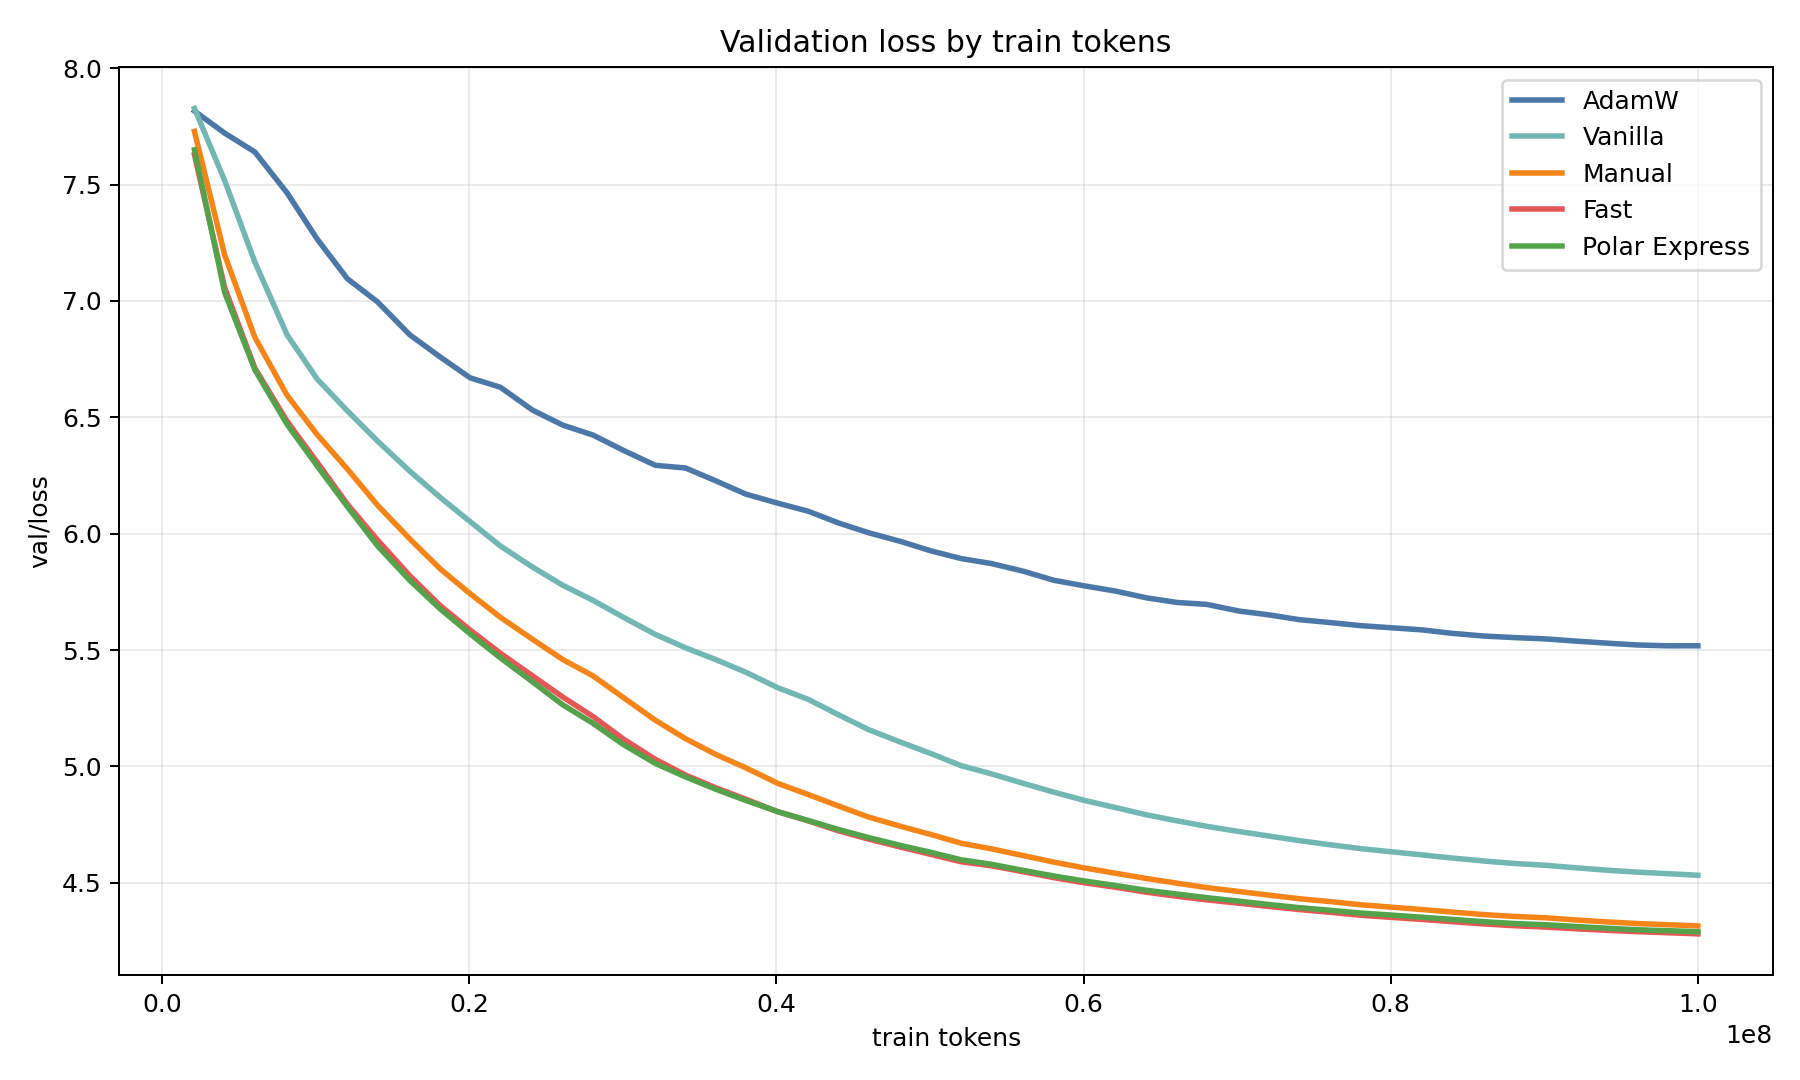
\includegraphics[width=\linewidth]{figures/val_loss_vs_tokens.png}
    \caption{Validation loss versus tokens.}
\end{subfigure}\hfill
\begin{subfigure}[t]{0.48\textwidth}
    \centering
    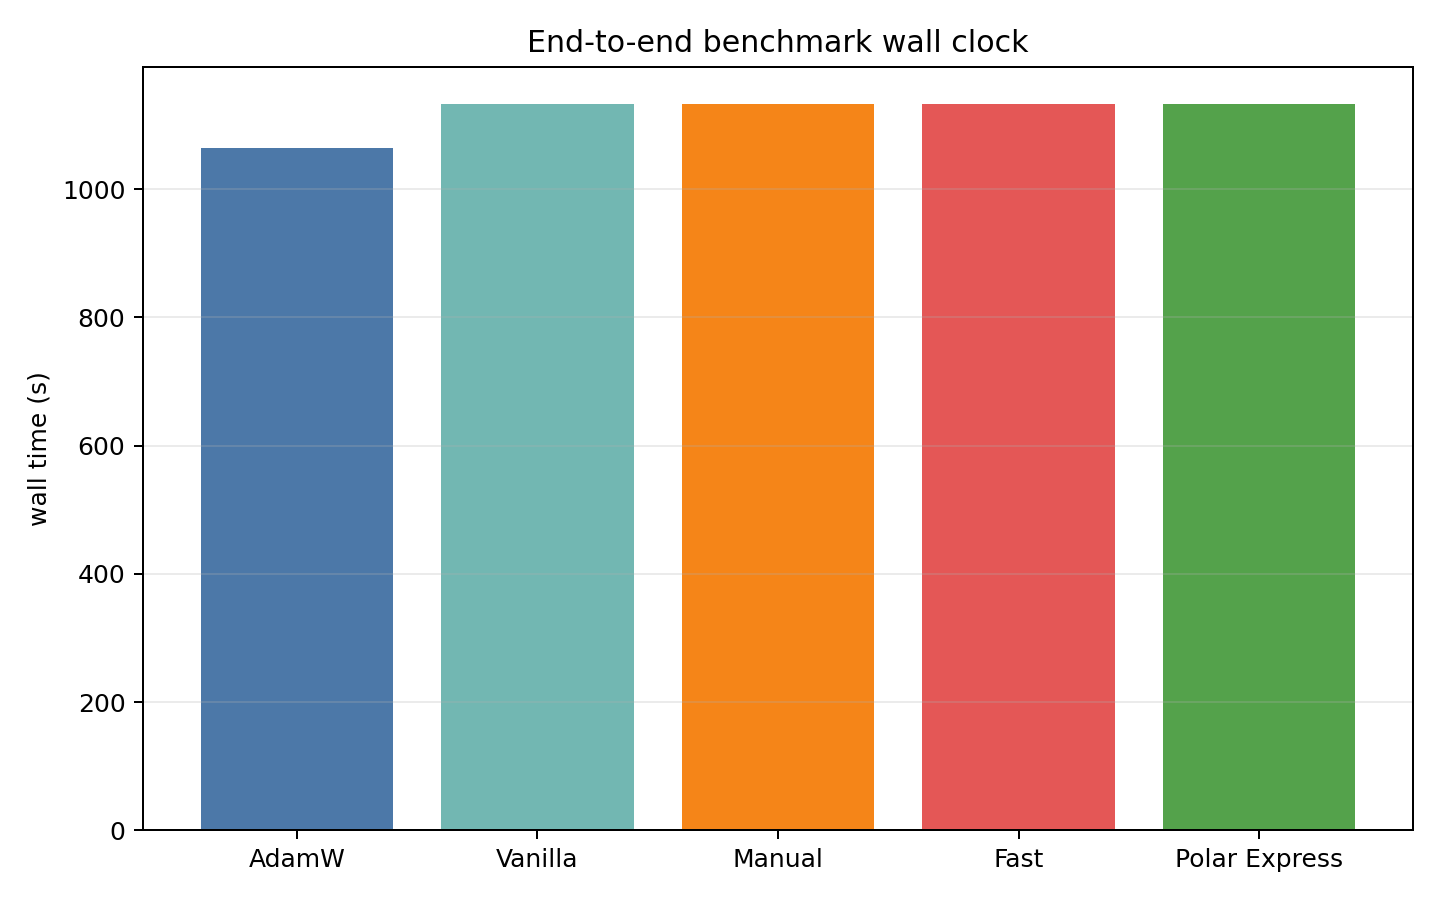
\includegraphics[width=\linewidth]{figures/benchmark_wall_clock.png}
    \caption{End-to-end wall-clock benchmark.}
\end{subfigure}

\vspace{0.5em}

\begin{subfigure}[t]{0.48\textwidth}
    \centering
    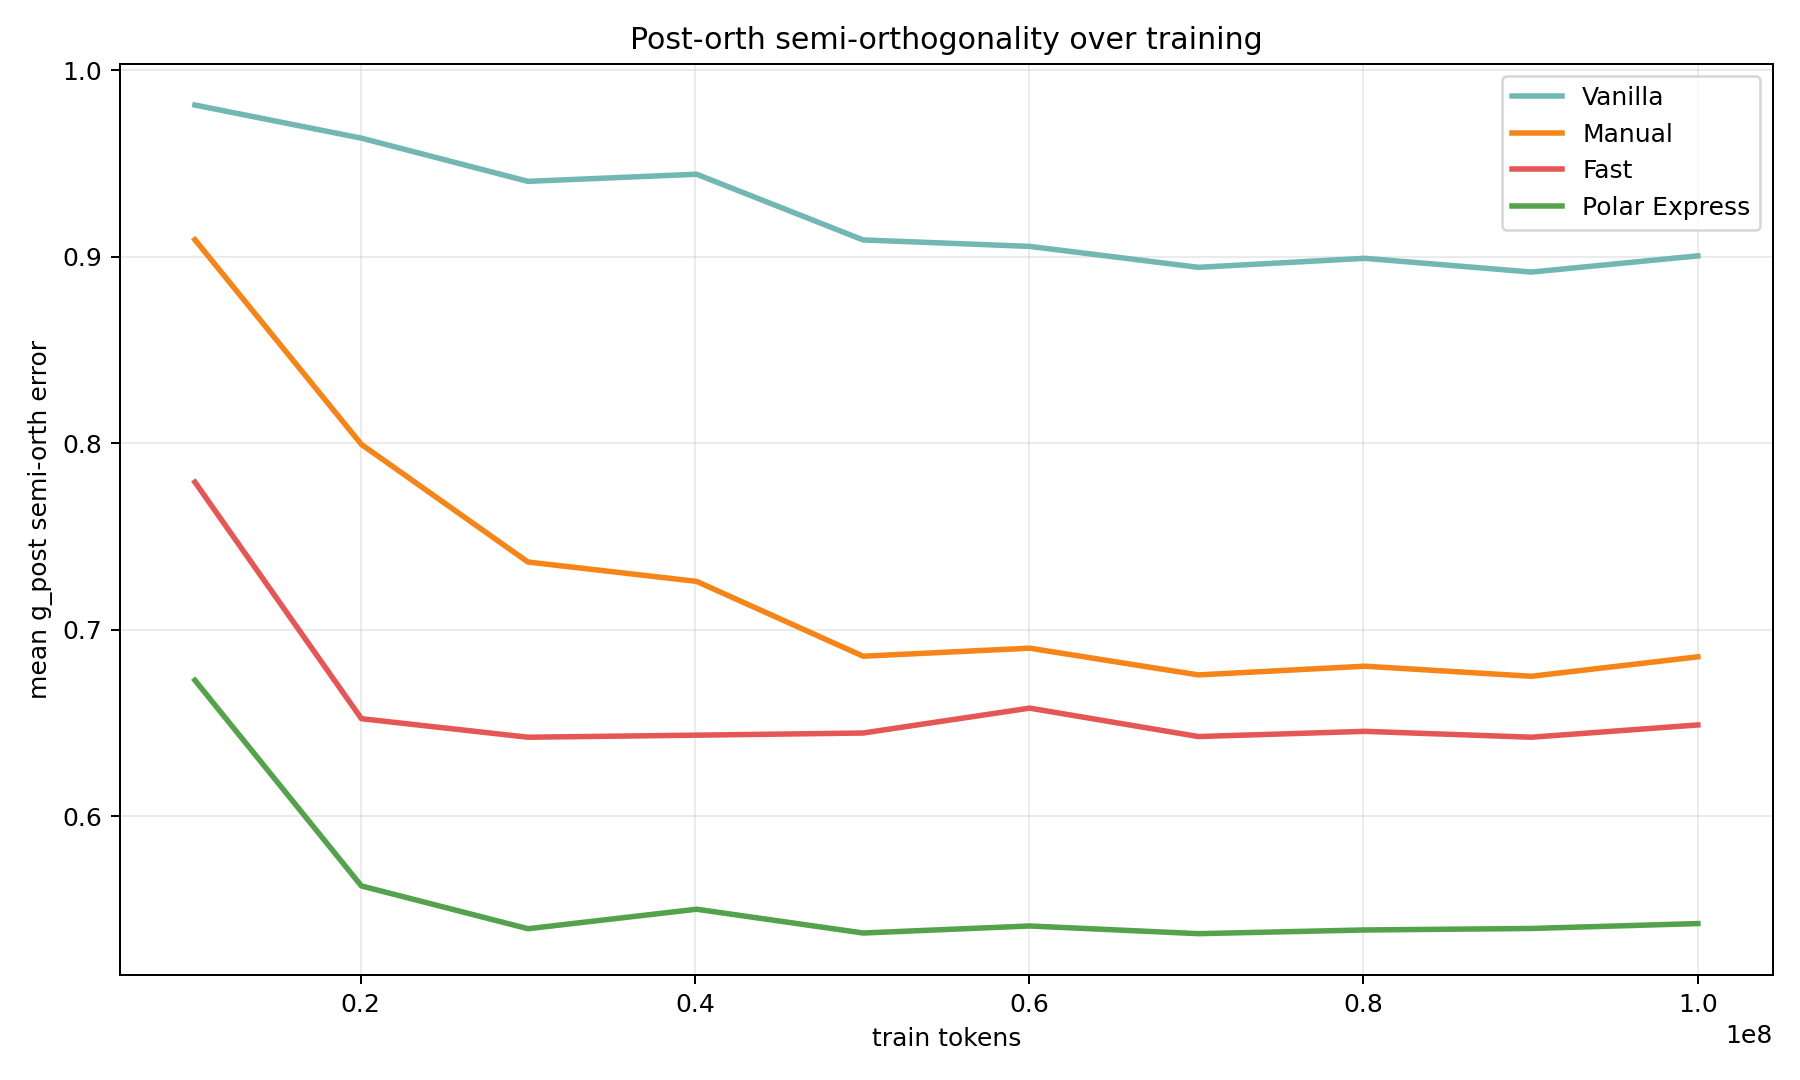
\includegraphics[width=\linewidth]{figures/g_post_semi_orth_error_vs_tokens.png}
    \caption{$\texttt{g\_post}$ semi-orthogonality over training.}
\end{subfigure}\hfill
\begin{subfigure}[t]{0.48\textwidth}
    \centering
    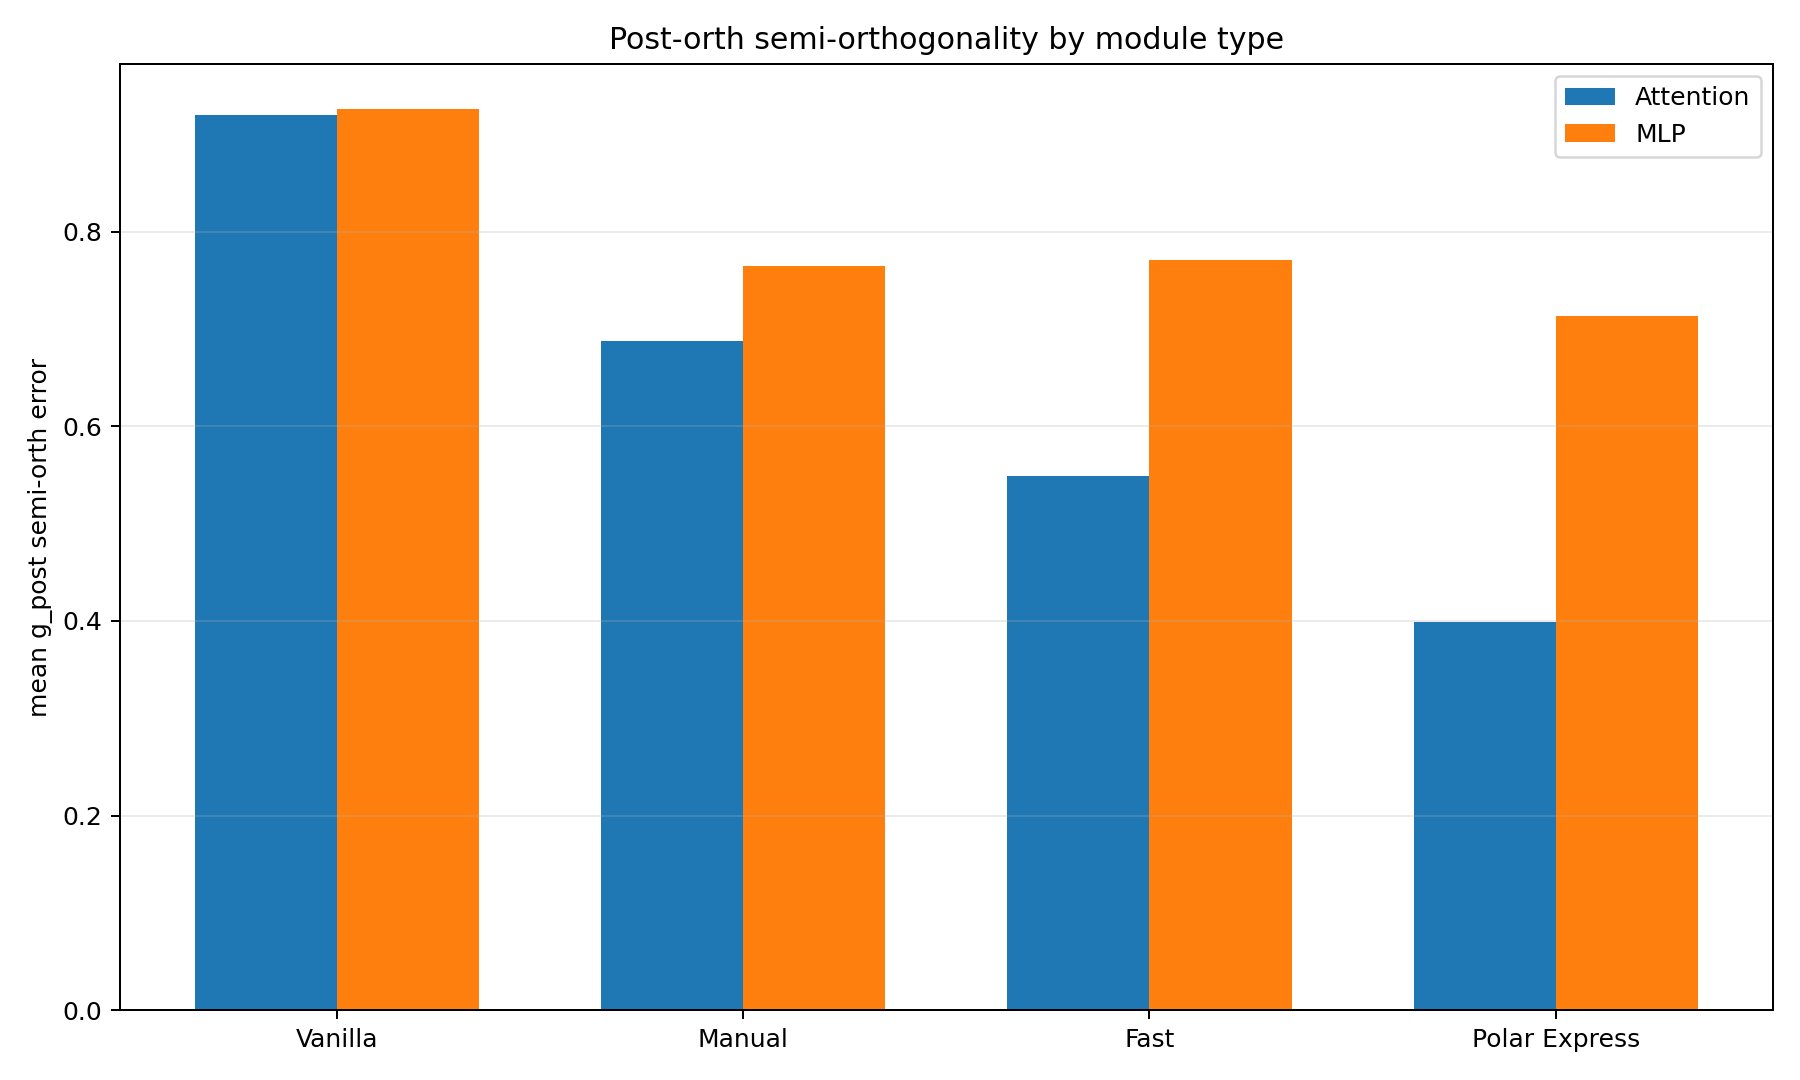
\includegraphics[width=\linewidth]{figures/g_post_semi_orth_error_attn_vs_mlp.png}
    \caption{Attention vs.\ MLP semi-orthogonality.}
\end{subfigure}
\caption{Main empirical evidence. The training and spectral rankings are consistent, while benchmark differences inside the Muon family are negligible.}
\label{fig:main}
\end{figure*}

Figure~\ref{fig:main} summarizes the full story. Fast and Polar Express separate early from Vanilla in both convergence and geometry, and their geometric advantage persists throughout training. Meanwhile, the wall-clock plot remains nearly flat across all Muon schedules, confirming that schedule choice is primarily a geometric and optimization question rather than a throughput question in this codebase.

\section{Conclusion}
This project studied Muon as a family of NS-defined spectral transformations rather than as a single optimizer. Under a fixed GPT pretraining stack, the coefficient schedule has a clear and reproducible effect on both update geometry and training quality. The most important empirical conclusion is that \textbf{better post-orthogonalization geometry usually corresponds to better pretraining behavior}: Polar Express produces the most semi-orthogonal updates, while Fast gives the best final validation loss and remains nearly tied with Polar Express throughout training.

The project also clarifies what does \emph{not} change. Within the Muon family, coefficient schedules have essentially identical end-to-end runtime, so the practical tradeoff is not ``fast schedule vs.\ slow schedule'' in wall-clock terms. Instead, it is a tradeoff between different spectral maps that induce different optimization trajectories.

\textbf{Limitations.}
The report should be interpreted with several constraints in mind:
\begin{itemize}
    \item all results use a single seed, so sensitivity to random initialization is not measured;
    \item the study fixes one model scale, one token budget, and one data pipeline;
    \item AdamW is included as a baseline rather than as a fully re-tuned competing optimizer;
    \item the spectral analysis is a sampled diagnostic, not a full SVD of every update matrix.
\end{itemize}

\textbf{Future directions.}
The next natural step is a multi-seed study of the strongest schedules, especially Fast and Polar Express, to determine whether their small loss gap is statistically meaningful. A second direction is to extend the mathematical analysis of the composed quintic map, connecting fixed points, contraction regions, and lower-bound assumptions more directly to the observed attention-dominant spectral differences. More broadly, the project suggests that NS schedule design is a promising optimization-geometry problem in its own right.

\begingroup
\footnotesize
\setlength{\bibsep}{1.5pt}
\bibliographystyle{abbrvnat}
\bibliography{references}
\endgroup

\end{document}
